\documentclass[a5paper,titlepage,10pt,openany]{scrbook}
\usepackage[a5paper,backref]{hyperref}
\usepackage[papersize={148.5mm,215mm},twoside,bindingoffset=0.5cm,hmargin={2cm,2cm},
				vmargin={2cm,2cm},footskip=1.1cm,driver=dvipdfm]{geometry}
\usepackage{palatino}
\usepackage{pstricks}
\usepackage{graphicx}
\usepackage[bahasa]{babel} 
%\usepackage[pdftex]{dropping}
\usepackage{lettrine}
\usepackage{pifont}
\usepackage{enumitem}
\usepackage{wrapfig}
\usepackage{indentfirst}
\usepackage{parcolumns}
\usepackage[titles]{tocloft}
\usepackage{longtable}
%\usepackage[raggedright]{titlesec}
%\usepackage{titletoc}


\renewcommand{\cftchapfont}{%
  \fontsize{9}{8}\selectfont
}

\makeatletter
\renewcommand{\@pnumwidth}{1em} 
\renewcommand{\@tocrmarg}{1em}
\makeatother

\author{Lingkungan St. Petrus Maguwo}
\title{Warta Iman}
\setlength{\parindent}{1cm}
\psset{unit=1mm}

\makeatletter
\renewcommand{\@makeschapterhead}[1]{%
  {\parindent \z@ \centering \normalfont
    \interlinepenalty\@M \Large \bfseries #1\par\nobreak \vskip 20\p@ }}
\renewcommand{\section}{\@startsection {section}{1}{\z@}%
                                   {-3.5ex \@plus -1ex \@minus -.2ex}%
                                   {2.3ex \@plus.2ex}%
%                                   {\normalfont\normalsize\bfseries\centering}}
                                   {\normalfont\normalsize\bfseries}}
\renewcommand\subsection{\@startsection{subsection}{2}{\z@}%
                                     {-3.25ex\@plus -1ex \@minus -.2ex}%
                                     {1.5ex \@plus .2ex}%
                                     {\normalfont\normalsize\bfseries}}
\renewcommand\subsubsection{\@startsection{subsubsection}{3}{\parindent}%
                                    {3.25ex \@plus1ex \@minus.2ex}%
                                    {-1em}%
                                    {\normalfont\normalsize\bfseries}}

\makeatother

\makeatletter  % Allow the use of @ in command names
\long\def\@makecaption#1#2{%
  \vskip\abovecaptionskip
  \sbox\@tempboxa{{#1#2}}%
  \ifdim \wd\@tempboxa >\hsize
    {#1#2\par}
  \else
    \hbox to\hsize{\hfil\box\@tempboxa\hfil}%
  \fi
  \vskip\belowcaptionskip}
\makeatother   % Cancel the effect of \makeatletter

\newcommand{\chap}[1]{%
    \chapter*{#1}
	\addcontentsline{toc}{chapter}{#1}
    }

\newcommand{\sumber}[1]{%    
	\begin{flushright}
	{\emph{#1}}
	\end{flushright}
}
\newcommand{\qti}[1]{%    
	\begin{quote}
	{\emph{#1}}
	\end{quote}
}

\hyphenation{sa-u-da-ra-ku}
\hyphenation{ke-ri-ngat}
\hyphenation{je-ri-tan}
\hyphenation{hu-bung-an}
\hyphenation{me-nya-dari}
\hyphenation{Eng-kau}
\hyphenation{ke-sa-lah-an}
\hyphenation{ba-gai-ma-na}
\hyphenation{Tu-han}
\hyphenation{di-per-ca-ya-kan}
\hyphenation{men-ja-uh-kan}
\hyphenation{bu-kan-lah}
\hyphenation{per-sa-tu-kan-lah}
\hyphenation{ma-khluk}
\hyphenation{Sem-buh-kan-lah}
\hyphenation{ja-lan}
\hyphenation{mem-bu-tuh-kan}
\hyphenation{be-ri-kan-lah}
\hyphenation{me-ra-sa-kan}
\hyphenation{te-man-ilah}
\hyphenation{mem-bi-ngung-kan}
\hyphenation{di-ka-gum-i}
\hyphenation{ta-ngis-an-Mu}
\hyphenation{mi-lik-ilah}

\renewcommand{\figurename}{~}
\renewcommand\thefigure{~}

\setlist{noitemsep}
\renewcommand{\thesection}{\Alph{section}}

\begin{document}
\thispagestyle{empty}
\thispagestyle{empty}
\newcommand{\edisi}[1]{%
\DeclareFixedFont{\PT}{T1}{ppl}{b}{}{0.7in}
\DeclareFixedFont{\PTit}{T1}{ppl}{b}{it}{0.7in}
\DeclareFixedFont{\PTsmall}{T1}{ppl}{b}{it}{0.25in}
\DeclareFixedFont{\PTsmaller}{T1}{ppl}{b}{it}{0.175in}
\DeclareFixedFont{\PTsmallest}{T1}{ppl}{b}{it}{0.15in}

\begin{pspicture}(14cm,2cm)
\rput[rb](10.35cm,3cm){\PTsmallest {#1}}
\rput[lb](-2cm,1.5cm){\PT {WARTA IMAN}}
\rput[lb](0cm,0.5cm){\PTsmall {Lingkungan St. Petrus Maguwo}}
\end{pspicture}%
}

\newcounter{kgkcounter}[chapter]
\renewcommand{\thekgkcounter}{\arabic{kgkcounter}. }
\newcommand{\kgk}[1]{\refstepcounter{kgkcounter}\textbf{\flushleft \textbf{\thekgkcounter #1}}\\}

\newcommand{\kutipan}[1]{%
\noindent{\framebox{\parbox{10cm}{\centering\emph{#1}}}}}

\edisi{November 2011}

%\vspace{1cm}

\begin{center}
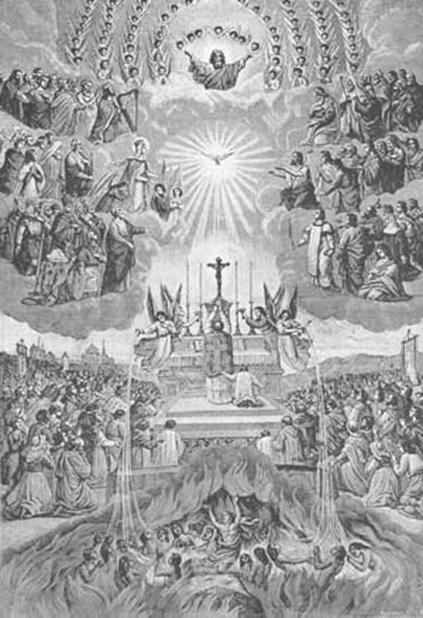
\includegraphics[scale=0.85]{gambar/purgatory2.jpg}
\end{center}

%\vspace{1cm}

\begin{center}
{\PTsmaller {Kasih, kerendahan hati, dan menurut pada kehendak Allah }}
\end{center}

\setlength{\parindent}{1cm}
\pagestyle{plain}
%\chap{Pemahaman Perkawinan Menurut Gereja Katolik}


\section*{Ajaran Gereja Katolik Tentang Perkawinan}

Ada begitu banyak pasangan calon mempelai yang sudah lama ber­pacaran, namun seringkali mereka belum mempergunakan kesempatan pacaran itu untuk dapat mempersiapkan diri dalam membangun keluarga katolik. Salah satu hal yang sangat penting namun seringkali terlupakan adalah kurangnya/ tidak pernah dilaksanakan pengolahan pengalaman hidup untuk melangsungkan suatu pernikahan sesuai ajaran Gereja Katolik. Oleh karena itu pentinglah, dalam membaca uraian di bawah ini, pembaca menggali pengalaman pribadi, khususnya ketika mempersiapkan perkawinannya. Rumusan ini bisa membantu un­tuk menilai diri sendiri, apakah memang sudah siap (minimal) secara mental dan rohani untuk melangsungkan perkawinan.

\noindent{Perkawinan adalah}
\begin{quote}
\begin{enumerate}[label=\Alph*.]
\item PERSEKUTUAN HIDUP  
\item ANTARA SEORANG PRIA DAN SEORANG WANITA  
\item YANG TERJADI KARENA PERSETUJUAN PRIBADI  
\item YANG TAK DAPAT DITA­RIK KEMBALI 
\item DAN HARUS DIARAHKAN 
\item KEPADA SALING MENCINTAI SEBAGAI SUAMI ISTERI 
\item DAN KEPADA PEMBANGUNAN KELUARGA 
\item DAN OLEH KARENANYA MENUNTUT KESETIAAN YANG SEMPURNA 
\item DAN TIDAK MUNGKIN DIBATALKAN LAGI OLEH SIAPAPUN, 
\item KECUALI OLEH KEMATIAN.
\end{enumerate}
\end{quote}

\section{Persekutuan hidup}
Apa yang pertama-tama kelihatan pada perkawinan Katolik? Jawabnya adalah: Hidup bersama. Namun, hidup bersama itu masih berane­karagam isinya. Dalam perkawinan Katolik, hidup bersama itu mewujudkan persekutuan. Jadi, hidup bersama yang bersekutu. Bersekutu mengisyaratkan adanya semacam kontrak, semacam ikatan tertentu dengan sekutunya. Bersekutu mengandaikan juga kesediaan pribadi untuk melaksanakan persekutuan itu, dan untuk menjaga persekutuan itu. Ada kesediaan pribadi untuk mengikatkan diri kepada sekutunya, dan ada kesediaan pribadi untuk memperkembangkan ikatannya itu supaya menjadi semakin erat.

Ikatan ini tidak mengurangi kebebasannya. Justru ikatan itu mengisi kebebasan orang yang bersangkutan. Pertama-tama karena para calon mempelai memilih sendiri untuk bersekutu, dan bebas un­tuk memilih mau bersekutu dengan siapa, memilih untuk terikat dengan menggunakan kebebasan sepenuhnya; tetapi juga karena kebebasan itu hanya dapat terlaksana dalam melaksanakan pilihannya untuk bersekutu ini. Dengan kata lain boleh dikatakan bahwa persekutuan itu membuat orang sungguh-sungguh bebas karena dapat memperkem­bangkan kreatifitas dalam memelihara dan mengembangkan persekutuan itu; bukan dengan menghadapkan diri pada pilihan-pilihan yang baru lagi. Persekutuan yang dibangun itu menjadi tugas kehidupan yang harus dihayatinya.


\section{Seorang pria dengan seorang wanita}
Penekanan pertama di sini adalah seorang dengan seorang: arti­nya orang seutuhnya dengan orang seutuhnya. Ini menggambarkan penerimaan terhadap satu pribadi seutuhnya. Yang diterima untuk bersekutu adalah pribadi, bukan kecantikan, kegantengan, kekayaan atau kepandaiannya saja. Ada beberapa catatan untuk penerimaan satu pribadi ini: Pertama, menerima pribadi itu berarti menerima juga seluruh latar belakang dan menerima seluruh masa depannya. Artinya, saya tidak dapat menerima pribadi itu hanya sebagai satu pribadi yang berdiri sendiri. Selalu, saya harus menerima juga orang tuanya, kakak dan adiknya, saudara-saudaranya, teman-teman­nya, bahkan juga bahwa dia pernah berpacaran atau bertunangan dengan si ini atau si itu. Lebih jauh lagi, saya juga harus meneri­ma segala sesuatu yang terjadi padanya di masa mendatang: syukur kalau ia menjadi semakin baik, tetapi juga kalau ia menjadi sema­kin buruk karena penyakit, karena ketuaan, karena halangan-halangan; saya masih tetap harus menerimanya. Yang ke dua, menerima pribadi berarti menerima dia apa adanya, dengan segala kelebihan dan kekurangannya. Kalau dipikir secara matematis: yang berseku­tu itu satu dengan satu; bukan $\frac{3}{4} + \frac{1}{2}$, atau $1 + \frac{6}{7}$; lebih-le­bih lagi, bukan 1 dengan $1\frac{1}{2}$, $1\frac{1}{4}$, atau $1\frac{3}{4}$, apalagi dengan 2, 3, dan seterusnya.

Dengan ungkapan lain lagi: Saya seutuhnya, mau mencintai dia seutuhnya/apa adanya. Ini berarti, saya mau menerima dia seutuh­nya, apa adanya; tetapi juga sekaligus saya mau menyerahkan diri seutuhnya kepadanya saja. Yang lain sudah tidak mendapat tempat lagi di hati saya, di pikiran saya. Hanya dia saja. Bahkan, anak-anakpun tidak boleh melebihi dia di hadapan saya, dalam pelayanan saya.
Penekanan ke dua pada seorang pria dengan seorang wanita.Yang ini kiranya cukup jelas. Hanya yang sungguh-sungguh pria dan yang sungguh-sungguh wanita yang dapat melaksanakan perkawinan secara katolik.


\section{Persekutuan pribadi}
Hidup bersekutu itu terjadi karena setuju secara pribadi. Yang harus setuju adalah yang akan menikah. Dan persetujuan itu dilakukan secara pribadi, tidak tergantung pada siapapun, bahkan juga pada pasangannya. Maka, rumusannya yang tepat adalah: “Saya setu­ju untuk melangsungkan pernikahan ini, tidak peduli orang lain setuju atau tidak, bahkan tidak peduli juga pasangan saya setuju atau tidak”.
“Lalu bagaimana kalau pasangan saya kurang atau bahkan tidak setuju?. Dia hanya pura-pura setuju”. Kalau demikian, bukankah pihak yang setuju dapat dirugikan? Ya, inilah resiko cinta sejati. Cinta sejati di sini berarti saya setuju untuk mengikatkan diri dengan pasangan, saya setuju untuk menyerahkan diri kepada pasangan, saya setuju untuk menjaminkan diri pada pasangan; juga kalau akhirnya persetujuan saya ini tidak ditanggapi dengan baik/sesuai dengan kehendak saya. Yang menjadi dasar pemahaman ini adalah karena setiap mempelai membawa cinta Kristus sendiri. Kristuspun tanpa syarat mengasihi kita, Kristus tanpa syarat menerima kita dan memberikan DiriNya bagi kita.

\section{Persetujuan pribadi yang tak dapat ditarik kembali}
Persetujuan pribadi untuk bersekutu itu nilainya sama dengan sumpah/janji dan bersifat mengikat seumur hidup. Sebab persetujuan itu mengikutsertakan seluruh kehendak, pikiran, kemauan, pera­saan. Pokoknya seluruh kepribadian. Maka dinyatakan bahwa perse­tujuan itu tidak dapat ditarik kembali. Sebab, penarikan kembali pertama-tama berarti pengingkaran terhadap diri sendiri, penging­karan terhadap kebebasannya sendiri, pengingkaran terhadap cita-cita dan kehendaknya sendiri. Tetapi, kemudian, juga berarti bah­wa pribadinya sudah tidak menjadi utuh kembali.

\section{Dan yang diarahkan}
Sebenarnya, pengalaman untuk membuat dan memelihara dan memper kembangkan persetujuan pribadi untuk bersekutu itu sudah harus dipupuk sejak masa pacaran Maka, ada banyak yang merasa bahwa persetujuan semacam itu sudah tidak perlu dipertanyakan lagi. Pokok­nya sudah beres, begitu. Semua sudah siap. Namun, kenyataannya persetujuan yang terjadi pada masa pacaran belumlah memenuhi sya­rat perkawinan. Dan benarlah, persetujuan yang dibangun pada masa pacaran baiklah persetujuan sebagai pacar. Persetujuan yang dibangun pada masa tunangan, baiklah persetujuan sebagai tunangan. Baru, setelah menikah, persetujuan itu boleh menjadi persetujuan sebagai suami-isteri. Maka, Kita lihat, misalnya adanya pembatasan-pembatasan dalam berpacaran, menunjukkan bahwa persetujuan itu belum bisa dilaksanakan sepenuhnya. Secara lebih positif dapat dikatakan bahwa persetujuan semasa pacaran lebih diarahkan untuk dapat melaksanakan janji pada saat perkawinan. Supaya janji pada saat perkawinan sungguh berisi dan memberi jaminan bagi masa de­pan baik pribadi maupun pasangannya. Tiga kata ini juga dapat diartikan penegasan terhadap perkawi­nan sebagai awal dari kehidupan baru bagi kedua mempelai. Bagai­manapun oleh perubahan situasi manusia masih dapat berubah. Pene­gasan ini membantu para suami/isteri untuk melaksanakan isi persetujuan itu.

\section{Saling mencintai sebagai suami isteri}
Pengalaman menunjukkan bahwa calon mempelai biasanya bingung dengan ungkapan ini. Mereka merasa sudah saling mencintai, kok masih ditanya soal ini. Masalahnya, sering tidak disadari bahwa cinta itu bermacam-macam. Ada cinta sebagai saudara, ada cinta sebagai sahabat, ada cinta karena belas kasihan, demikian pula ada cinta suami isteri. Tentu saja, yang namanya cinta sejati tidak pernah dapat berbeda-beda. Yesus menunjuk cinta sejati itu seba­gai orang yang mengorbankan nyawaNya bagi yang dicintaiNya. Dan Yesus memberi teladan dengan hidupNya sendiri yang rela sengsa­ra, bahkan sampai wafat untuk kita semua yang dicintaiNya. Na­mun, perwujudan cinta sejati itu ternyata bisa beranekaragam. Kekhasan dari cinta suami isteri adalah adanya keterikatan isti­mewa yang membuat mereka dapat menyerahkan diri seutuhnya bagi pasangannya. Dalam hal ini kiranya cinta suami isteri dapat diseja­jarkan dengan cinta yang diwujudkan dalam suatu kaul biara atau janji seorang imam. Bedanya, kalau kaul biara atau janji seorang imam tertuju kepada Tuhan di dalam umatNya; dalam perkawinan cinta itu tertuju kepada Tuhan di dalam pasangannya. Yang mau dituju adalah membangun suasana saling mencintai sebagai suami/isteri. Maka, tidak hanya membabi buta dengan cintanya sendiri. “Pokoknya saya sudah mencintai”. Ini tidak cukup. Perjuangan seorang suami/isteri adalah di samping memelihara dan memperkembangkan cintanya, juga mengusahakan supaya pasangannya da­pat ikut mengembangkan cintanya sebagai suami/isteri.

\section{Pembangunan keluarga}
Hidup dalam persekutuan sebagai suami-isteri mau tidak mau mewujudkan suatu keluarga. Harus siap untuk menerima kedatangan anak-anak, harus siap untuk tampil sebagai keluarga, baik di hadapan saudara-saudara, di hadapan orang tua maupun di hadapan masya­rakat pada umumnya. Maka, membangun hidup sebagai suami-isteri membawa juga kewajiban untuk mampu menghadapi siapapun sebagai satu kesatuan dengan pasangannya. Mampu bekerjasama menerima, meme­lihara dan mendewasakan anak, mampu bekerjasama menerima atau da­tang bertamu kepada keluarga-keluarga lain, mampu ikut serta mem­bangun Gereja. Semuanya dilaksanakan dalam suasana kekeluargaan.

\section{Kesetiaan yang sempurna}
Setia dalam hal apa? Empat hal yang sudah diuraikan di atas, yakni persekutuan hidup antara seorang pria dan seorang wanita, memelihara dan memperkembangkan persetujuan pribadi, membangun sa ling mencintai sebagai suami isteri, membangun hidup berkeluarga yang sehat. Tidak melaksanakan salah satunya berarti sudah tidak setia. Apalagi kalau kemudian mengalihkan perhatiannya kepada se­suatu yang lain: membangun persekutuan yang lain, membuat perse­tujuan pribadi yang lain, membangun hubungan saling mencintai sebagai suami isteri dengan orang lain, membangun suasana kekeluargaan dengan orang lain (juga saudara): Ini dosanya besar sekali
Satu pedoman untuk kesetiaan yang sempurna adalah Kristus sen­diri. Ia setia kepada tugas perutusanNya, Ia setia kepada Bapa­Nya, Ia setia kepada manusia, kendati manusia tidak setia kepadaNya.

\section{Tak dapat dipisahkan oleh siapapun}
Persekutuan perkawinan terjadi oleh dua pihak, yakni oleh sua­mi dan isteri. Maka, tidak ada instansi atau siapapun yang akan dapat memutuskan persetujuan pribadi itu. Bahkan suami isteri itu sendiripun tidak dapat memutuskannya, sebab persekutuan itu dibangun atas dasar kehendak Tuhan sendiri. Dan Tuhanlah yang merestuinya. Maka, pemutusan persekutuan perkawinan bisa dipandang sebagai pemotongan kehidupan pribadi suami/isteri. Ini bisa be­rarti pembunuhan, karena pribadi itu dihancurkan.

\section{Kecuali oleh kematian}
Pengecualian ini didengar tidak enak. Namun, nyatanya, misteri kematian tidak terhindarkan. Karena kematian yang wajar, persetu­juan pribadi itu menjadi batal, karena pribadi yang satu sudah tidak mampu lagi secara manusiawi melaksanakan persetujuannya. 

\sumber{http://www.imankatolik.or.id}
\chap{Sakramen Perkawinan: sebuah usaha untuk memahami secara ``baru''}

\begin{center} \textit{Blasius Slamet Lasmunadi, Pr} \end{center}

\small
    Usaha memahami Sakramen Perkawinan secara ``baru'' ini saya gulirkan
    dalam beberapa tulisan. Mengapa ``secara baru'', karena gagasan ini
    saya tuangkan dalam rangka memperdalam gagasan retret para imam
    Keuskupan Purwokerto (10-14 Nov 2008) di Purwokerto bersama Fr Fio
    Mascarenhas dari India, yang menekan pentingnya relasi umat beriman
    dengan Tritunggal Mahakudus.
    	
    Saya menempatkan status diri dalam tulisan ini sebagai seorang
    imam dan sebagai  seorang anak dalam keluargaku. Karena itu tulisan
    saya ini barangkali banyak bernuansa teologis daripada praksis.
    Justru karena kurang praksis, terbukalah kesempatan untuk Anda
    semua, untuk mengkritik tulisan ini atau memberi komentar apapun,
    juga yang ``nakal'' sekalipun dipersilakan.
    Tulisan ini dibagi menjadi 2 bagian: (A) Suami isteri sebagai mitra
    kerja Allah dan (B) Peran suami isteri sebagai imam, nabi dan raja.
\normalsize

\section{Suami isteri sebagai ``mitra rekan kerja Allah''}
    Dalam Perayaan Sakramen Pernikahan, kita sering mendengarkan Sabda
    Tuhan yang diwartakan seperti ini, ``\textit{Sebab pada awal dunia, Allah
    menjadikan mereka laki-laki dan perempuan,sebab itu laki-laki akan
    meninggalkan ayahnya dan ibunya dan bersatu dengan
    isterinya,sehingga keduanya itu menjadi satu daging. Demikianlah
    mereka bukan lagi dua, melainkan satu. Karena itu, apa yang telah
    dipersatukan Allah, tidak boleh diceraikan manusia (Mrk 10:6-9)}''
    
    Sabda Tuhan yang menegaskan kebersatuan suami isteri itu dan sifat
    monogaminya, juga ditegaskan dalam Kitab Hukum Kanonik 1983, kan. 1056:\\
    ``\textit{Ciri-ciri hakiki perkawinan ialah unitas (kesatuan=monogami) dan
    indissolubilitas/ (sifat tak-dapat-diputuskan), yang dalam
    perkawinan kristiani memperoleh kekukuhan khusus atas dasar sakramen.}''
    
    Sifat monogami dan sifat tak dapat diputuskan itu tentulah
    dimengerti oleh para calon suami isteri sebelum mereka mengucapkan
    kesepakatan janji nikah. Janji nikah yang diucapkan pria dan wanita
    yanga dibaptis, dan diucapkan di hadapan Allah dan Gereja, mereka
    berdua telah ``saling menerimakan sakramen perkawinan''. Kesepakatan
    nikah pria dan wanita yang dibuat  dengan tahu, sadar dan bebas dari
    segala paksaan apapun, adalah keputusan untuk ``menjadi mitra Allah''
    dalam karya keselamatan-Nya.

    Suami isteri menjadi ``mitra Allah'' dengan hidup dalam persekutuan
    sebagai ``Gereja keluarga''. Apakah artinya ``persekutuan'' bagi suami
    isteri? Artinya, saat mengucapkan janji nikah di hadapan Allah dan
    Gereja, suami isteri saling ``menukar'' hidup dan pribadinya. Suami
    menyatakan ``engkau isteriku, seluruh dirimu kugantikan dengan
    diriku''. Demikian juga isteri bersedia ``engkau suamiku, seluruh
    dirimu kugantikan dengan diriku''. Maka dengan pertukaran itu, suami
    dapat memandang dan memperlakukan isterinya, sebagai ``dirinya
    sendiri'' , sebaliknya begitu. Dengan kata lain, suami isteri saling
    mengarahkan jerih payahnya untuk hidup pasangannya, bukan hidup
    dirinya sendiri. Itulah ``mengasihi sesama seperti dirinya sendiri''
    dalam keluarga. Kasih antar sesama itu dapat menjadi ``tanda kasih''
    yang hidup dari kesetiaan kasih Allah kepada manusia.
    
    Allah Bapa tidak menyesal menciptakan manusia, meskipun Adam dan
    Hawa, akhirnya jatuh dalam dosa asal. Keturunan merekapun satu per
    satu, bergantian, turun temurun, dari generasi satu ke generasi yang
    lain, mewarisi dosa asal. Maka setelah melalui sejarah yang
    berliku-liku, Allah mengutus Putera-Nya yang tunggal, Yesus untuk
    hidup dan tinggal bersama manusia.

    Kristus itulah yang melaksanakan tugas untuk menebus dosa manusia,
    dengan hidup dan wafat-Nya di kayu salib. Tugas itu dilaksanakan
    dengan sempurna oleh Kristus sehingga Allah tidak segan untuk
    meninggikan ``Dia di atas segala nama'', dengan membangkitkan-Nya pada
    hari ketiga. Kebangkitan itu menganugerahkan kebebasan sebagai
    anak-anak Allah. Akan tetapi kebebasan itu tidak serta merta
    ditanggapi manusia untuk hidup di dalam Roh, mengasihi Allah dan
    sesama, malahan kerap kali kebebasan itu disalahgunakan untuk
    ``bekerjasama dengan kuasa kegelapan dosa'', yakni hidup menurut
    daging. Karena itulah, Yesus mengutus Roh-Nya sendiri setelah 50
    hari kebangkitan-Nya agar manusia mampu memenangkan pertempuran
    antara kehendak untuk hidup dalam Roh dan kecenderungan hidup dalam
    kegelapan dosa.
    
    Dengan lain kata, keputusan pria dan wanita untuk hidup menikah,
    adalah buah Roh Kudus, yakni menggunakan kebebasannya sebagai anak
    Allah untuk mewujudkan panggilan dasarnya sebagai citra dan anak-Nya
    untuk mencintai seperti Allah mencintai manusia. Panggilan dasar itu
    diwujudkan dalam hidup pernikahan. Maka sakramen pernikahan
    memperbaharui buah buah sakramen pembaptisan. Buah sakramen
    pembaptisan, tidak hanya mendapat anugerah kebebasan sebagai anak
    Allah, melainkan juga memberi daya kekuatan untuk menggulirkan
    kebebasan itu dalam tiga perannya: sebagai imam, nabi dan raja.

     

\section{Tiga peran Suami Isteri dalam kemitraan dengan Allah}

    Suami isteri kristiani sebagai orang yang dibaptis telah
    dipercaya menjadi anak-Nya sekaligus ahli waris. Karena itu mereka
    dipanggil untuk menjadi \textbf{imam}, \textbf{nabi} dan \textbf{raja}.
     
    \textbf{Sebagai imam}, suami isteri dipanggil untuk membangun relasi yang
    intim dengan Allah. Relasi itu dibangun dengan ``merayakan iman'' dan
    ``mewujudkan iman dalam tindakan kasih.'' Tugas merayakan iman adalah
    kesediaan untuk berdoa: berbicara dengan Tuhan dalam berbagai macam
    kesempatan. Termasuk juga, yang harus dibuat, belajar minta Roh
    Kudus kepada Allah Bapa karena Roh Kudus tidak otomatis
    dianugerahkan kepada kita, melainkan Ia akan hadir dan terlibat
    dalam hidup kita.

\begin{quote}
    \textit{Jadi jika kamu yang jahat tahu memberi pemberian yang baik kepada
    anak-anakmu, apalagi Bapamu yang di sorga! Ia akan memberikan Roh
    Kudus kepada mereka yang meminta kepada-Nya (Luk 11, 13)}
\end{quote}


    Roh Kudus sudah hadir di tengah tengah kita, namun bagaimana kita
    mampu mengalami karya Roh itu kalau tidak membuka diri. Ibarat
    bagaikan orang yang mencari sinar matahari di pagi hari sampai
    siang, padahal dia terus menerus tinggal di gua dan tidak pernah mau
    keluar dari gua itu. Maka, penting dan mendesak, jangan ragu-ragu
    untuk meminta Roh Kudus kepada Bapa agar terlibat membantu
    memberikan pencerahan di saat banyak kesulitan.

    Sikap hidup ``yang melibatkan Roh'' itu pasti akhirnya menantang
    suami isteri untuk  melepaskan diri dari ketergantungan terhadap 
    fasilitas yang nampaknya dapat diandalkan. Dengan lain kata,
    melibatkan Roh dalam hidup bersama, berarti  jerih payah apapun
    suami isteri dapat menjadi korban persembahan bagi Tuhan kalau
    dilaksanakan demi kepentingan terwujudnya buah-buah Roh, ``\textit{kasih,
    sukacita, damai sejahtera, kesabaran, kemurahan, kebaikan,
    kesetiaan, kelemahlembutan, penguasaan diri.' (Gal 5:22-23)}''
    
    Sebaliknya jerih payah suami isteri, bahkan yang kelihatan luhur
    sekalipun tidak akan menjadi "kurban persembahan bagi Allah" kalau
    dilaksanakan demi "kepentingan sendiri" atau demi kepentingan
    "daging". Karena hidup dalam daging, ``\textit{percabulan, kecemaran, hawa
    nafsu,  penyembahan berhala, sihir, perseteruan, perselisihan, iri
    hati, amarah, kepentingan diri sendiri, percideraan, roh
    pemecah,kedengkian, kemabukan, pesta pora dan sebagainya (Gal 5: 21)}''

    Dengan kata lain \textbf{peran sebagai imam menuntut peran sebagai "raja"},
    yang memiliki sikap "proaktif untuk melayani sesamanya". Mereka
    tidak akan berbangga kalau menjadi pribadi yang suka disapa, atau
    jadi pribadi yang ditakuti pasangan hidup atau anaknya sendiri. 
    Allah sendiri menganugerahkan Roh sebagai anak Allah bukan roh
    perbudakan yang membuat kita takut."\textit{Semua orang, yang dipimpin Roh
    Allah, adalah anak Allah.Sebab kamu tidak menerima roh perbudakan
    yang membuat kamu menjadi takut lagi, tetapi kamu telah menerima Roh
    yang menjadikan kamu anak Allah. Oleh Roh itu kita berseru: 'ya
    Abba, ya Bapa!' (Rm 8:14-15)}"  Dengan keyakinan Santo Paulus ini,
    suami isteri dipanggil untuk menampilkan hidup sebagai anak Allah.
    Hidup sebagai anak Allah selalu terarah pada kepentingan Bapa, dan
    bukan kepentingan harga diri sendiri. Maka, suami isteri mesti
    belajar untuk dinilai dan dikritik oleh pasangannya. Kalau keliru,
    belajar cepat meminta maaf, tidak malahan membela diri dan
    berargumentasi bahwa dirinya benar. Kalaupun benar pendapatnya,
    lebih baik mengatakan, "Terima kasih atas kritikanmu! Iya, bisa jadi
    saya keliru, meski sekarang saya yakin pendapatku ini benar!"
    Keterbukaan seperti itulah, yang meningkatkan kualitas pribadi yang
    siap untuk diubah oleh Roh Kudus.  Dengan semangat itu, suami isteri
    dapat mewujudkan sakramen perkawinan: sebagai tanda kehadiran cinta
    Tuhan yang nyata, yakni,
\small
\begin{enumerate}[label=(\roman*) ]
\item menjadi tanda cinta Allah Bapa Sang Pencipta dan pemelihara
    hidup melalui prokreasi, merawat dan mendidik anak sampai mandiri,

\item menjadi tanda kasih Yesus yang menebus dosa manusia dengan
    mengampuni satu sama lain, tidak menghakimi, namun belajar untuk
    mengubah kelemahan pasangan menjadi kesempatan untuk berefleksi dan

\item belajar untuk menjadi tanda kehadiran Roh Kudus yang menyertai
    kita sepanjang hidup, dengan belajar mendengarkan dan berkanjang
    bersama: tidak saling melempar kesalahan, tidak saling melempar
    tanggung jawab, melainkan belajar setia, yakni sehati seperasaan
    dalam suka dan duka.
\end{enumerate}
\normalsize
    Ketiga tindakan itu berwarna Trinitaris, maka ketiga tindakan itu
    tidak terpisahkan. Tidak cukup pasutri hanya prokreasi dan mendidik
    anak tanpa pengampunan dan solider antara suami isteri dan antar
    orang tua dan anak. Dengan cara hidup macam seperti suami isteri
    menjadi "tanda cinta yang hidup dari kesetiaan Allah kepada manusia".
    Akan tetapi bagaimana penghayatan itu sampai pada kenyataan kalau
    suami isteri kurang membuka diri kepada sabda Allah. \textbf{Karena itu
    peran sebagai imam dan raja, mesti didukung dengan peran sebagai
    nabi, yang bersedia mendengarkan sabda Allah dan melaksanakan dalam
    hidup setiap hari.} Sabda Tuhan itu adalah roh dan kehidupan. Maka
    suami isteri ditantang untuk hidup dari Sabda agar mereka memiliki
    "roh dan kehidupan" karena ``\textit{Perkataan-perkataan yang Kukatakan
    kepadamu adalah roh dan hidup.}'' (Yoh 6:63). itulah sebabnya Petrus
    pun setia mengikuti kemana Yesus pergi karena "Perkataan-Mu adalah
    perkataan hidup yang kekal"/ (Yoh 6:68). Kata-kata Yesus itu sendiri
    meneguhkan kita semua, agar tidak lagi ragu-ragu untuk setia
    mendengarkan Sabda Tuhan agar kita mengenal siapa Kristus, dan
    terlebih agar kita memiliki roh dan hidup!! Maka suami isteri
    ditantang untuk sungguh berperan sebagai "nabi": menjadi tanda
    kehadiran Allah yang bersabda bagi pasangannya, anak-anaknya dan
    saudara-saudarinya.
    
    Dengan penghayatan begitulah, pasutri membawa hidupnya dalam
    persembaan di altar dalam ekaristi. Hidupnya dengan segala kerapuhan
    dan kelemahan dipersembahkan bersama kurban Kristus, agar saat
    komuni terjadilah "pertukaran ilahi": Kristus hadir dalam diri suami
    isteri  untuk menerima hati mereka dengan segala keletihan dan rasa
    lesu serta beban berat, dan menggantikannya dengan  Tubuh dan
    Darah-Nya, agar setelah ekaristi, hidup mereka dalam keluarga
    sungguh menampilkan hidup Kristus yang setia pada Gereja-Nya. 
    Karena itu Kristus yang setia pada Gereja-Nya membutuhkan suami
    isteri untuk bekerjasama, agar kesetiaan Kristus tampak bagi dunia. 
    Di situlah tugas suami isteri, "menampakkan" kesetiaan kasih Kristus
    bagi dunia.
    
    Dengan "menampakkan kesetiaan" itu dalam hidup bersama yang diwarnai
    kasih, suami isteri menjadi tanda "pertukaran ilahi" antara Kristus
    dengan manusia. Itulah "pertukaran" yang menjadi ciri khas
    "persekutuan suami isteri monogami dan tidak terceraikan". Semoga
    makin banyak pasutri kristiani yang menjadi tanda kasih Allah yang
    hidup bagi dunia.

    Salam hangat untuk pasutri dan keluarga kristiani di manapun berada.

    \sumber{Blasius Slamet Lasmunadi, Pr\\http://www.imankatolik.or.id/}
\normalsize
\chap{Prosedur Pernikahan Gereja Katolik}
\setlist{noitemsep}

\section{Tahap pertama}
\begin{enumerate}
\item   Pendaftaran pernikahan di Gereja melalui sekretariat pada paroki masing-masing pada hari kerja (hari kerja dan waktu buka seketariat disesuaikan masing-masing paroki
\item    Membawa surat pengantar dari lingkungan calon mempelai (baik pria dan wanitanya). Dalam hal ini surat pengantar untuk mengikuti KPP (Kursus Persiapan Perkawinan)
\item    Membawa fotokopi surat baptis yang diperbaharui :
\begin{enumerate}
    \item    Katolik dengan non Katolik - salah satu calon mempelai yang beragama Katolik
    \item    Katolik dengan Katolik – kedua calon mempelai wajib melampirkannya
\end{enumerate}

   Surat baptis yang diperbaharui berlaku 6 bulan samapai dengan hari H (pernikahannya)

\item    Membawa pasfoto 3x4 masing-masing 3 lembar
\item    Menyelesaikann biaya administrasi KPP (Kursus Persiapan Pernikahan), besar biaya disesuaikan paroki masing-masing. Hal-hal yang berkaitan dengan pendaftaran KPP, bisa ditanyakan di sekretariat masing-masing paroki.
\end{enumerate}

\section{Tahan Kedua}
\begin{enumerate}
\item   Selesaikan prosedur Tahap Pertama
\item    Mengisi formulir dan menyerahkan berkas-berkas pernikahan,
    yaitu:
\begin{enumerate}
\item        Surat pengantar dari lingkungan masing--masing
\item        Sertifikat Kursus Persiapan Pernikahan yg asli dan fotokopinya
\item        Surat baptis asli yang telah diperbaharui
\item        Foto berwarna berdampingan ukuran 4x6 sebanyak 3 lembar
\item        Fotokopi KTP saksi pernikahan 2 (dua) orang yang Katolik
\end{enumerate}
\item    Kedua calon mempelai datang ke Romo ybs untuk melakukan pendaftaran penyelidikan kanonik (harus datang sendiri, tidak dapat diwakilkan)
\item    Bagi calon mempelai yang belum Katolik danlatau bukan Katolik, harap menghadirkan 2 (dua) orang saksi pada saat penyelidikan kanonik untuk menjelaskan status pihak yang bukan Katolik. Saksi adalah orang yang benar-benar mengenal pribadi calon mempelai yang bukan Katolik dan bukan anggota
    keluarga kandungnya.
\item    Apabila kedua calon mempelai dari luar Paroki/Gereja dimana domisili calon mempelai harap membawa surat delegasi/pelimpahan pemberkatan pernikahan dari Pastor/Romo setempat (tempat penyelidikan kanonik)
\end{enumerate}

\section{Pernikahan Catatan Sipil}
\begin{enumerate}
\item    Datang ke sekretariat Gereja sebulan sebelumnya untuk pengurusan pernikahan catatan sipil dengan membawa: (Bila catatan sipil dilakukan di Gereja setelah pernikahan)
\begin{enumerate}
\item        Surat pengantar dari Kelurahan untuk pendaftaran perkawinan
\item        Fotokopi KTP dan Kartu Keluarga kelurahan kedua belah pihak
\item        Fotokopi Akta Kelahiran kedua mempelai
\item        Fotokopi SKBRI (WNI). Jika tidak ada, bawa SKBRI/WNI orang tua
\item        Untuk umat keturunan - fotokopi surat ganti nama (Bila tidak ada, lampirkan surat ganti nama dari orangtua)  
\item        Pas foto berdampingan ukuran. 4 x 6 sebanyak 6 lembar
\end{enumerate}
\item    Akan dibuatkan pengumuman ke kantor Catatan Sipil sesuai KTP yang bersangkutan dari calon mempelai. (kebijakan ini tergantung catatan sipil setempat)
\item    Pada hari "H", Akta Kelahiran asli kedua mempelai dan Surat Pemberkatan Nikah Gereja diserahkan kepada petugas Catatan Sipil
\item    Pencatatan pernikahan sipil bisa diurus oleh mempelai sendiri atau oleh pihak Gereja.
\end{enumerate}

\chap{Kebijakan Paroki Tentang Pernikahan Pada Masa Khusus}
    Pada prinsipnya gereja dilarang merayakan misa ritual pada hari Minggu selama masa khusus. Aturan ini tercantum dalam \textit{Misale Romanum} terbaru art. 372. beberapa hal yang harus diperhatikan melalui pernyataan di atas adalah:

\begin{enumerate}
\item    Misa ritual adalah perayaan yang berkaitan dengan sakramen (mis: pernikahan) atau sakramentali (pemberkatan rumah).
\item  Masa khusus meliputi:
\begin{enumerate}
\item    Adven
\item    Rabu Abu
\item    Prapaskah
\item    Pekan Suci (Minggu Palma - Kamis Putih - Jumat Agung -  Sabtu Suci -Malam Paskah - Minggu Paskah)
\item     Minggu Palma
\item Kamis Putih

\item Jumat Agung
\item Sabtu Suci
\item Malam Paskah
\item Paskah
\item OktafPaskah
\item Peringatan arwah semua orang beriman (setiap tgl. 02 November)          
\end{enumerate}
\end{enumerate}


    Berdasarkan makna dan suasana masa khusus dari dua dokumen liturgi, yaitu: \textit{Misale Romanum} dan \textit{Litterae Circurales De Festis Paschalibus Praeparandis et Celebrands}, biasanya ada kebijakan (tergantung paroki setempat) berkaitan dengan perayaan upacara pernikahan, sbb:
\begin{enumerate}
\item    Dalam masa Adven dan Prapaskah masih diijinkan untuk melangsungkan upacara pernikahan dengan memperhatikan kesederhanaan. Ukuran kesederhanaannya adalah:
\begin{enumerate}
\item \textbf{Masa Adven}

    Gereja

\begin{itemize}
\item        Hiasan bunga diijinkan hanya di sekitar altar.
\item        Tidak menggunakan karpet di lorong.
\item        Tidak ada hiasan bunga di sepanjang lorong menuju altar.
\item        Tidak ada hiasan bunga di pintu masuk gereja.
\item        Warna liturgi mengikuti masa yang berlaku
\end{itemize}

    Imam dan mempelai

\begin{itemize}
\item        Kasula imam berwarna putih.
\item        Mempelai diperkenankan membawa bunga tangan.
\item        Diperkenankan mempersembahkan bunga di patung Maria.
\end{itemize}

\item \textbf{Masa prapaskah}

    Gereja

\begin{itemize}
\item        Hiasan bunga TIDAK DIIJINKAN sama sekali dan diganti
\item        dengan dedaunan secukupnya di sekitar altar.
\item        Tidak menggunakan karpet di lorong
\item        Tidak ada hiasan bunga di sepanjang lorong menuju altar
\item        Tidak ada hiasan bunga di pintu masuk gereja
\item        Warna liturgi mengikuti masa yang berlaku
\item        Organ/alat musik lainnya hanya bersifat mengiringi lagu (tidak ada instrumental)
\item        Lagu-Iagu juga tidak sebanyak masa liturgi umum (dikonsultasikan dengan imam)
\end{itemize}

    Imam dan mempelai
\begin{itemize}
\item        Kasula imam berwarna putih
\item        Mempelai diperkenankan membawa bunga tangan
\item        Diperkenankan mempersembahkan bunga di patung Maria
\end{itemize}
\end{enumerate}

\item Dalam upacara Rabu abu, pekan suci, oktaf paskah, dan peringatan arwah semua orang beriman 2 November TIDAK DIIJINKAN untuk melangsungkan upacara pernikahan.

\item Kebijakan ini akan berubah (bersifat tentatif) setelah dokumen khusus tentang pernikahan dari KWI mendapat pengesahan dari Vatikan dan diberlakukan di Keuskupan-keuskupan di Indonesia.
\end{enumerate}
\chap{Halangan yang Menggagalkan Perkawinan}

\setcounter{section}{0}
\section{Kurangnya umur (bdk. kan 1083):}

Syarat umur yang dituntut oleh kodeks 1983 adalah laki-laki berumur 16 tahun dan perempuan berumur 14 tahun dan bukan kematangan badaniah. Tetapi hukum kodrati menuntut kemampuan menggunakan akalbudi dan mengadakan penilaian secukupnya dan ``\textit{corpus suo tempore habile ad matrimonium}''. Hukum sipil sering mempunyai tuntutan umur lebih tinggi untuk perkawinan dari pada yang dituntut hukum Gereja. Jika salah satu pihak belum mencapai umur yang ditentukan hukum sipil, Ordinaris wilayah harus diminta nasehatnya dan izinnya diperlukan sebelum perkawinan itu bisa dilaksanakan secara sah (bdk kan. 1071, \S1, no.3). Izin semacam itu juga harus diperoleh dari Ordinaris wilayah dalam kasus di mana orang tua calon mempelai yang belum cukup umur itu tidak mengetahui atau secara masuk akal tidak menyetujui perkawinan itu (bdk. kan 1071, \S1, no.6).

\section{Impotensi (bdk kan. 1084):}

Impotensi itu adalah halangan yang menggagalkan, demi hukum kodrati, dalam perkawinan. Sebab impotensi itu mencegah suami dan istri mewujudkan kepenuhan persatuan hetero seksual dari seluruh hidup, badan dan jiwa yang menjadi ciri khas perkawinan. Yang membuat khas persatuan hidup suami istri adalah penyempurnaan hubungan itu lewat tindakan mengadakan hubungan seksual dalam cara yang wajar. Impotensi yang menggagalkan perkawinan, haruslah sudah ada sebelum perkawinan dan bersifat tetap. Pada waktu perkawinan sudah ada, bersifat tetap maksudnya impotensi itu terus menerus dan bukan berkala, serta tidak dapat diobati kecuali dengan operasi tidak berbahaya. Impotensi ada dua jenis: bersifat absolut dan relatif. Impotensi absolut jika laki-laki atau perempuan sama sekali impotens. Impotensi relatif jika laki-laki atau perempuan tertentu ini tidak dapat melaksanakan hubungan seksual. Dalam hal absolut orang itu tidak dapat menikah sama sekali, dalam impotensi relatif pasangan tertentu juga tidak dapat menikah secara sah.

\section{Adanya ikatan perkawinan (bdk. kan 1085):}

Ikatan perkawinan terdahulu menjadi halangan yang menggagalkan karena hukum ilahi. Kan 1085, \S1: menghilangkan ungkapan “kecuali dalam hal privilegi iman” (Jika dibandingkan dengan kodeks 1917). Ungkapan ini berarti jika seorang yang dibaptis menggunakan privilegi iman walau masih terikat oleh ikatan perkawinan terdahulu, dia bisa melaksanakan perkawinan secara sah dan ketika perkawinan baru itu dilaksanakan ikatan perkawinan lama diputuskan.

\section{Disparitas cultus (bdk. kan 1086):}

Perkawinan antara dua orang yang diantaranya satu telah dibaptis dalam Gereja Katolik atau diterima di dalamnya dan tidak meninggalkannya dengan tindakan formal, sedangkan yang lain tidak dibaptis, adalah tidak sah. Perlu dicermati ungkapan “meninggalkan Gereja secara formal” berarti melakukan suatu tindakan yang jelas menunjukkan etikat untuk tidak menjadi anggota Gereja lagi. Tindakan itu seperti menjadi warga Gereja bukan Katolik atau agama Kristen, membuat suatu pernyataan di hadapan negara bahwa dia bukan lagi Katolik. Namun demikian janganlah disamakan tindakan itu dengan orang yang tidak pergi ke Gereja Katolik lagi tidak berarti meninggalkan Gereja. Ada dua alasan tentang norma ini: pertama karena tujuan halangan ini adalah untuk menjaga iman katolik, tidak ada alasan mengapa orang yang sudah meninggalkan Gereja harus diikat dengan halangan itu. Kedua, Gereja tidak mau membatasi hak orang untuk menikah.

Perkawinan yang melibatkan disparitas cultus (beda agama) ini, sesungguhnya tetap dapat dianggap sah, asalkan: 1) sebelumnya pasangan memohon dispensasi kepada pihak Ordinaris wilayah/ keuskupan di mana perkawinan akan diteguhkan. Dengan dispensasi ini, maka perkawinan pasangan yang satu Katolik dan yang lainnya bukan Katolik dan bukan Kristen tersebut tetap dapat dikatakan sah dan tak terceraikan; setelah pihak yang Katolik berjanji untuk tetap setia dalam iman Katolik dan mendidik anak-anak secara Katolik; dan janji ini harus diketahui oleh pihak yang non-Katolik (lih. kan 1125). 2) Atau, jika pada saat sebelum menikah pasangan tidak mengetahui bahwa harus memohon dispensasi ke pihak Ordinaris, maka sesudah menikah, pasangan dapat melakukan \textit{Convalidatio} (lih. kann. 1156-1160) di hadapan imam, agar kemudian perkawinan menjadi sah di mata Gereja Katolik.

\section{Tahbisan suci (bdk. kan. 1087):}

Adalah tidak sahlah perkawinan yang dicoba dilangsungkan oleh mereka yang telah menerima tahbisan suci.
Kaul kemurnian dalam suatu tarekat religius (bdk. kan. 1088):

Kaul kekal kemurnian secara publik yang dilaksanakan dalam suatu tarekat religius dapat menggagalkan perkawinan yang mereka lakukan.

\section{Penculikan dan penahanan (bdk. kan. 1089):}

Antara laki-laki dan perempuan yang diculik atau sekurang-kurangnya ditahan dengan maksud untuk dinikahi, tidak dapat ada perkawinan, kecuali bila kemudian setelah perempuan itu dipisahkan dari penculiknya serta berada di tempat yang aman dan merdeka, dengan kemauannya sendiri memilih perkawinan itu. Bahkan jika perempuan sepakat menikah, perkawinan itu tetap tidak sah, bukan karena kesepakatannya tetapi karena keadaannya yakni diculik dan tidak dipisahkan dari si penculik atau ditahan bertentangan dengan kehendaknya.

\section{Kejahatan (bdk. kan. 1090):}

Tidak sahlah perkawinan yang dicoba dilangsungkan oleh orang yang dengan maksud untuk menikahi orang tertentu melakukan pembunuhan terhadap pasangan orang itu atau terhadap pasangannya sendiri.

\section{Persaudaraan (konsanguinitas (bdk. kan. 1091):}

Alasan untuk halangan ini adalah bahwa perkawinan antara mereka yang berhubungan dalam tingkat ke satu  garis lurus bertentangan dengan hukum kodrati. Hukum Gereja merang perkawinan di tingkat lain dalam garis menyamping, sebab melakukan perkawinan di antara mereka yang mempunyai hubungan darah itu bertentangan dengan kebahagiaan sosial dan moral suami-isteri itu sendiri dan kesehatan fisik dan mental anak-anak mereka.

\section{Hubungan semenda (bdk. kan. 1092):}

Hubungan semenda dalam garis lurus menggagalkan perkawinan dalam tingkat manapun. Kesemendaan adalah hubungan yang timbul akibat dari perkawinan sah entah hanya ratum atau ratum consummatum. Kesemendaan yang timbul dari perkawinan sah antara dia orang tidak dibaptis akan menjadi halangan pada hukum Gereja bagi pihak yang mempunyai hubungan kesemendaan setelah pembaptisan dari salah satu atau kedua orang itu. Menurut hukum Gereja hubungan kesemendaan muncul hanya antara suami dengan saudara-saaudari dari isteri dan antara isteri dengan saudara-saaudara suami. Saudara-saudara suami tidak mempunyai kesemendaan dengan saudara-saudara isteri dan sebaliknya. Menurut kodeks baru 1983 hubungan kesemendaan yang membuat perkawinan tidak sah hanya dalam garis lurus dalam semua tingkat.

\section{Halangan kelayakan publik (bdk. kan. 1093):}

Halangan ini muncul dari perkawinan tidak sah yakni perkawinan yang dilaksanakan menurut tata peneguhan yang dituntut hukum, tetapi menjadi tidak sah karena alasan tertentu, misalanya cacat dalam tata peneguhan. Halangan ini muncul juga dari konkubinat yang diketahui publik. Konkubinat adalah seorang laki-laki dan perempuan hidup bersama tanpa perkawinan atau sekurang-kurangnya memiliki hubungan tetap untuk melakukan persetubuhan kendati tidak hidup bersama dalam satu rumah. Konkubinat dikatakan publik kalau dengan mudah diketahui banyak orang.

\section{Adopsi (bdk. kan. 1094):}

Tidak dapat menikah satu sama lain  dengan sah mereka yang mempunyai pertalian hukum yang timbul dari adopsi dalam garis lurus atau garis menyamping tingkat kedua. Menurut norma ini pihak yang mengadopsi dihalangi untuk menikah dengan anak yang diadopsi, dan anak yang diadopsi dihalangi untuk menikah dengan anak-anak yang dilahirkan dari orang tua yang mengadopsi dia. Alasannya karena adopsi mereka menjadi saudara-saudari se keturunan.
\chap{Ciri-ciri Perkawinan Katolik}

Sebagai penggambaran persatuan ilahi antara Kristus dengan Gereja-Nya, Perkawinan Katolik mempunyai tiga ciri yang khas, yaitu ikatan 
\begin{enumerate}
\item yang \textbf{terus berlangsung seumur hidup}, 
\item \textbf{monogami}, yaitu satu suami, dan satu istri, 
\item yang \textbf{tidak terceraikan}. 
\end{enumerate}
Sifat terakhir inilah yang menjadi ciri utama perkawinan Katolik. Di dalam ikatan Perkawinan ini, suami dan istri yang telah dibaptis menyatakan kesepakatan mereka, untuk saling memberi dan saling menerima, dan \textbf{Allah sendiri memeteraikan kesepakatan ini}. Perjanjian suami istri ini digabungkan dengan perjanjian Allah dengan manusia, dan karena itu cinta kasih suami istri diangkat ke dalam cinta kasih Ilahi. Atas dasar inilah, maka Perkawinan Katolik yang sudah diresmikan dan dilaksanakan tidak dapat diceraikan. Ikatan perkawinan yang diperoleh dari keputusan bebas suami istri, dan telah dilaksanakan, tidak dapat ditarik kembali. \textbf{Gereja tidak berkuasa untuk mengubah penetapan kebijaksanaan Allah ini}.

Karena janji penyertaan Allah ini, dari ikatan perkawinan tercurahlah juga berkat-berkat Tuhan yang juga menjadi persyaratan perkawinan, yaitu berkat untuk menjadikan perkawinan tak terceraikan, berkat kesetiaan untuk saling memberikan diri seutuhnya, dan berkat keterbukaan terhadap kesuburan akan kelahiran keturunan. \textbf{Kristus-lah sumber rahmat dan berkat ini}. Yesus sendiri, melalui sakramen Perkawinan, menyambut pasangan suami istri. Ia tinggal bersama-sama mereka untuk memberi kekuatan di saat-saat yang sulit, untuk memanggul salib, bangun setelah jatuh, saling mengasihi dan mengampuni.

Maka, apa yang dianggap mustahil oleh dunia, yaitu setia seumur hidup kepada seorang manusia, menjadi mungkin di dalam Perkawinan yang mengikutsertakan Allah sebagai pemersatu. Ini merupakan kesaksian Kabar Gembira yang terpenting akan \textbf{kasih Allah yang tetap kepada manusia}, dan bahwa para suami dan istri mengambil bagian di dalam kasih ini. Betapa kita sendiri menyaksikan bahwa mereka yang mengandalkan Tuhan dalam perjuangan untuk saling setia di tengah kesulitan dan cobaan, sungguh menerima penyertaan dan pertolonganNya pada waktunya. Hanya kita patut bertanya, sudahkah kita mengandalkan Dia?
\chap{\textit{Cerpen:}\\Antara Permohonan dan Pilihan}

	Jika anda sering menonton celotehan selebriti di televisi, maka anda akan menemukan kisah-kisah lucu dan paradoksal. Terutama menyangkut hidup rumah tangga mereka. Pada saat diwawancarai menjelang pernikahan, betapa keduanya saling memberi pujian setinggi gunung. Dengan yakinnya mereka mengatakan bahwa Tuhan telah memberikan jodoh yang baik, cocok, penuh pengertian dan setia. Kitapun akan mengamini. Tetapi tidak sampai setahun setelah hari pernikahan mereka, pasangan itu tahu-tahu hadir lagi di Pengadilan Agama untuk mengurus  perceraian. Saat dikerubuti wartawan, masing-masing mengaku bahwa mereka sudah tidak ada kecocokan lagi. Perceraian adalah jalan terbaik daripada masing-masing menderita batin.

	Hal itu pula yang akan dilakukan oleh teman saya Thomas Joko Prayitno. Ia berniat akan menceraikan Yohanna istrinya. Alasannya mirip para selebriti yang mau cerai, tidak ada keharmonisan lagi. Hatiku turut merasakan prihatin. Joko dan Yohanna adalah teman karibku semasa kuliah dulu hingga sekarang kami tetap akrab.

``Kamu serius Jok?'' Tanya saya.

``Ya, setelah aku renung-renungkan, lebih baik kami cerai.'' Jawab Joko mantap. ``Seumpama piring, keluargaku adalah piring yang retak. Jadi tidak mungkin disatukan lagi.'' Lanjut Joko sambil menghela nafas panjang dan menggeleng-gelengkan kepalanya.

Saya tersenyum. ``Perumpamaan itu keliru besar. Hanya orang `\textit{p\'{e}thuk}'  yang mau menyamakan keluarganya sama dengan sebuah piring. ''

Mulut Joko ternganga. Ia kaget. ``Kamu menghina aku, Gung?'' bentak Joko emosi.

``Tenang kawan, sabar, sorry aku tidak bermaksud menghina kamu. Izinkan aku memberi penjelasan. Di dalam sebuah piring itu tidak ada Allah. Piring itu benda mati. Begitu pecah di buang ke keranjang sampah. Masih ingat dalam Injil ada Sabda yesus yang bunyinya begini: tetapi tentang kebangkitan orang-orang mati tidaklah kamu baca apa yang difirmankan Allah, ketika Ia bersabda: Akulah Allah Abraham, Allah Ishak dan Allah Yakub? Ia bukanlah Allah orang mati, melainkan Allah orang hidup. Jadi Allah kita tidak berkarya di benda mati seperti piring. Tetapi Dia berkarya di dalam diri kita, di dalam keluarga kita. Mengapa? Karena kita masih hidup, berarti masih punya jiwa, masih punya hati.'' Jelasku.

``Tetapi bagaimana jika dua hati sudah tidak bisa disatukan lagi?'' protesnya.

``Kamu masih ingat saat menerima Sakramen perkawinan di altar?'' tanyaku.

``Ya. Yang sudah dipersatukan oleh Allah tidak bisa diceraikan oleh manusia. Bukankah itu yang ingin kamu katakan? Ayat dari Kitab Suci itu memang bagus tujuannya, yakni hanya ada perkawinan sekali dalam hidup manusia. Tetapi bagaimana jika kami sudah tidak bisa harmonis lagi, tak ada kecocokan lagi. Setiap hari yang ada hanya cekcok mulut?'' tegas Joko.
Joko sedang terbakar emosinya. Seseorang dalam kondisi kejiwaan seperti itu tidak butuh nasehat. Justru nasehat bisa berubah menjadi minyak yang ditumpahkan ke bara api. Api akan membesar dan membakar semuanya.

``Hari Sabtu besok mau ikut saya?'' tanyaku setelah kami diam agak lama.

``Kemana?''

``Sudah lama saya ingin ke Sendangsono. Sudah lama saya tidak sowan Bunda Maria. Kangen rasanya.''
Joko mengangguk-angguk. Dan ia setuju mau ikut. Kami berangkat Sabtu pagi.

\section*{Jalan Salib penuh kenangan}

Hari itu saya dan Joko memulai jalan salib dari pemberhentian ke-1 di Gereja Promasan. Ajakannya untuk jalan salib rute pendek di Sendangsono saya tolak. Sebab itu jalan salibnya orang malas. Jalan salib yang tidak memberi inspirasi pada tubuh untuk sejenak ikut merasakan penderitaan Tuhan Yesus.
Menjelang, pemberhentian ke-VII kami berhenti. ``Masih ingat, apa yang kamu lakukan disini 18 tahun yang lalu?'' tanyaku pada Joko.

Joko diam. Terbayang kembali dalam ingatannya saat itu kondisi jalan untuk jalan salib di Sendangsono belum disemen seperti sekarang, masih dari tanah lempung, kalau hujan tanahnya akan ambles jika diinjak.  Malam itu Yohanna hampir jatuh, karena tanah yang diinjaknya ambles cukup dalam sehingga Yohanna tidak bisa lagi menjaga keseimbangan badannya hampir jatuh, lalu aku cepat-cepat merengkuh tangannya dan memeluknya erat-erat.

``Jok, masih ingat apa yang terjadi disini 18 tahun yang lalu?'' tanyaku lagi kepada Joko.

``Saat itu Yohanna hampir jatuh, lalu aku cepat-cepat merengkuh tangannya kemudian kupeluk erat-erat.'' Jawab Joko pelan.

Jalan salib kami lanjutkan lagi. Persis di pemberhentian ke-XII saya bertanya lagi, ``Masih ingat apa yang terjadi disini 18 tahun yang lalu?''
Joko mengangguk.

``Ada peristiwa apa?''

``Yohanna jatuh pingsan dalam pelukanku. Dia lalu `kubopong' dan kutidurkan di belakang warung itu. Setelah siuman, pelan-pelan dia `kupapah' sampai di Sendang. Meski tampak lemah, tapi dia kuat sampai disana.'' Kata Joko pelan.

Aku tersenyum. Doa jalan salib kami lanjutkan sampai di Sendang, kami bersimpuh di depan patung Bunda Maria. Selesai berdoa saya bertanya pada Joko, ``Apa yang kamu doakan 18 tahun yang lalu disini?''
Joko tidak segera menjawab. Ia mengambil nafas dalam-dalam, lalu berkata lirih, ``Aku minta Bunda Maria agar beliau mau menjadi perantara permohonanku kepada Tuhan Yesus.''

``Apa yang kamu mohon pada Tuhan Yesus?''

``Agar Dia mengijinkan Yohanna menjadi jodohku, menjadi isteriku. Menjadi ibu dari anak-anakku.''

``Dan Tuhan Yesus meluluskan permohonanmu, tidak?''

``Ya \ldots ya \ldots tetapi \ldots'' Joko tidak melanjutkan kalimatnya. Ada rombongan peziarah lain datang memenuhi pelataran di depan patung Bunda Maria.

\section*{Doa Peneguhan}

Seminggu kemudian, tanpa sepengetahuan Joko, Yohanna yang sudah kuanggap adik sendiri itu saya ajak ke Sendangsono. Kepada Yohanna saya ajukan pertanyaan yang sama seperti halnya Joko pada saat jalan salib. Dan jawabannya pun hampir sama mirip dengan jawaban suaminya Joko.

``Jadi Joko itu jodoh yang kamu minta kepada Tuhan Yesus dengan perantaraan  Bunda Maria?'' tanyaku pada Yohanna setelah selesai berdoa di depan patung Bunda Maria.
Yohanna mengangguk. 

Dua minggu kemudian keduanya saya ajak bersama-sama ke Sendangsono. Kami doa jalan salib bertiga, juga mulai dari pemberhentian ke-1 di Gereja Promasan. Menjelang pemberhentian ke-VII saya minta Yohanna untuk pura-pura jatuh seperti kejadian 18 tahun yang lalu. Dan Joko harus siap-siap menolongnya. Adegan itu berjalan dengan mulus. Yohanna jatuh ke dalam pelukan suaminya.

Di pemberhentian ke XII kembali saya minta Yohanna untuk pura-pura pingsan. Tetapi dia tidak mau. ``Malu!'' jawabnya. Namun saya terus membujuknya, sedikit mengancam bahwa saya akan pulang sendiri jika dia tetap menolak. Akhirnya yohanna menyerah. Dia pura-pura pingsan, lalu Joko membopong dan menidurkannya di belakang warung. Setelah itu Joko merangkul isterinya menuju ke pemberhentian ke-XV, lalu berdoa di depan patung Bunda Maria.

``Sekarang berdoalah seperti doa kalian 18 tahun yang lalu.'' Kata sayakemudian. ``Jangan berbohong. Sebab Bunda Maria dan Tuhan Yesus melihat kalian. Silahkan.'' Kata saya sambil mundur lalu duduk dibawah pohon beringin.
Saya tidak tahu apa yang mereka doakan. Sebab saya sendiri berdoa, memohon kepada Tuhan Yesus lewat perantaraan Bunda Maria, agar pasangan suami-isteri ini mengurungkan niatnya untuk berpisah. Bahtera oleng itu sudah biasa, namun jangan sampai menabrak karang dan hancur berkeping-keping.

Dua puluh menit kemudian saya dekati mereka berdua, saya sodorkan selembar kertas yang berisi doa tulisan tangan. Doa itu saya buat malam menjelang kami ziarah bersama. ``Tolong bacalah doa ini bersama-sama. Pelan-pelan saja. Bunda Maria pasti mendengar, begitu juga Tuhan Yesus.'' Saya lalu mundur dan duduk dibelakang keduanya sekitar jarak tiga meter.

Inilah doanya:
\begin{quote}\textit{
Allah Bapa yang maha rahim, Kami berdua duduk bersimpuh di depan Bunda Maria, kami berdua berpasrah diri depan Putra-Mu, Tuhan kami Yesus Kristus. 18 tahun yang lalu ya Tuhan, kami mengetuk kemurahan hati-Mu, dengan perantaraan bunda Maria, agar Engkau berkenan menyatukan dua hati kami menjadi suami-isteri dalam rumah tangga Kristiani. Engkau maha pemurah, maha mendengar, sebab kami pun boleh menerima Sakramen Perkawinan. Disaksikan para malaikat dan orang kudus, kami berjanji di depan –Mu untuk sehidup semati, dalam untung dan malang, tak terceraikan oleh manusia dan hukum mana pun, kecuali oleh maut. 
\bigskip\\ 
Namun ternyata dalam perjalanan mengayuh biduk, kami diterpa badai, diamuk ombak, haruskah kami karam di telaga kehidupan yang keras? Jika hal itu terjadi ya Tuhan, berarti kami tidak menghormati Dikau, tidak menghargai pemberian-Mu yang tak ternilai harganya, yakni pasangan hidup kami. 
\bigskip\\ 
Karena itu ya Tuhan, di depan Bunda Maria, kami berjanji untuk saling menjaga, tetap saling mencintai pasangan hidup kami, dengan kelebihan dan kekurangannya. Kami sadar bahwa tidak ada yang sempurna di dunia ini, kecuali kasih-Mu yang Engkau curahkan tanpa batas kepada kami. Bunda Maria berkatilah anak-anakmu ini. Mohonkan kepada Tuhan Yesus semangat memperbaharui hidup iman dan hidup cinta kasih kami. Amin.}
\end{quote}

Sebulan kemudian saya tidak bertemu dengan Joko dan Yohanna karena tugas pekerjaan harus keluar kota. Joko dan Yohanna memberi kabar bahwa mereka telah meninggalkan rumah orangtuanya. Keduanya sepakat untuk hidup mandiri, mengontrak rumah sederhana dan kecil. Kehidupan baru dimulai kembali, semoga Tuhan selalu berkenan hadir dalam keluarga mereka juga dalam  keluarga kita semua. Amin.

\sumber{Medio Januari '12\\Bravo Sierra}

\begin{center}
\bigskip

\includegraphics[scale=0.5]{gambar/wedding-4.jpg}
\end{center}
\chap{Warta Lingkungan}

\subsection*{APP}
Bulan Maret 2012 sudah masuk dalam masa Prapaskah. Sesuai dengan tradisi, setiap masa Prapaskah diadakan Aksi Puasa Pembangunan yang kegiatannya antara lain adalah ibadat APP di lingkungan. Untuk tahun ini Keuskupan Agung Semarang (KAS) menetapkan tema APP: \textit{Umat Katolik Sejati Harus Peduli dan Berbagi}. Dalam pelaksanaan di lingkungan St. Petrus, ibadat APP banyak diisi dengan \textit{sharing} yang mengacu pada buku panduan dari KAS.
Topik APP berawal dari baptis. Kapan kita dibaptis, kesan-kesan saat dibaptis, dan relevansinya dengan hidup menggereja dan bermasyarakat.

\subsection*{Misa pemberkatan rumah dan mitoni}
Bulan ini umat St. Petrus bertambah lagi dengan satu keluarga yang secara resmi bergabung sebagai warga lingkungan. Keluarga Bapak R. Mulyadi yang bertempat tinggal di Nanggulan, mengadakan misa syukur pemberkatan rumah dan sekaligus mitoni pada tanggal 22 Maret. Cicilia Nony Prayoga yang merupakan putri dari Bapak/Ibu Mulyadi menantikan kelahiran putranya bersama dengan suami tercinta
Bernadus Budhiprayoga.

Misa dipimpin oleh Rm. Albertus Purnomo, OFM yang merupakan kenalan baik keluarga R. Mulyadi saat masih di Jakarta. Dalam homilinya Romo menekankan bahwa Musa dapat melakukan tawar-menawar dengan Tuhan karena kedekatan Musa dengan Tuhan. Kenapa Musa dekat dengan Tuhan, karena Musa sering berdoa dan menaati perintah-Nya. Oleh karena itu kalau kita ingin dekat dengan Tuhan, maka rajin-rajinlah berdoa dan senantiasa menaati perintah-Nya.

\subsection*{Pendaftaran Krisma}
Telah diumumkan di gereja bahwa sakramen Krisma untuk paroki Marganingsih Kalasan akan dilangsungkan bulan September 2012. Calon penerima sakramen Krisma dapat mendaftarkan diri ke Ibu Munarti, Bapak Neo Suradi, atau kepada ketua lingkungan, dengan menyerahkan fotokopi surat baptis.

% SELECT day(`TglLahir`),
% concat(u1.`Baptis`,' ',u1.`Nama`) 
% FROM `umat` u1 WHERE month(TglLahir)=6 order by 1

%=========
% SELECT day(`TglNikah`),
% concat(u1.`Baptis`,' ',u1.`Nama`,' + ',u2.`Baptis`,' ',u2.`Nama`) 
% FROM `umat` u1 join kk on (u1.nokk=kk.id and u1.hubkel='KK')
%               join umat u2 on (u2.nokk=kk.id  and (u2.hubkel='istri' or u2.hubkel='isteri'))
% WHERE month(TglNikah)=1 order by 1

\section*{Yang berulang tahun kelahiran bulan ini}

\noindent{Semoga hari bahagia ini menguatkan imannya akan Dikau.}

\begin{longtable}{|c|l|} 
\hline
Tgl & Nama \\ \hline
\endhead1& Maria Rosary Sekar Seruni\\
5& Anna Maria Tri Henaningsih\\
6& Fransiscus Xaverius Sularto\\
7& Christina Sutarni\\
8& Marcellina Oktavia S. Padmini\\
11& Priscilla Oktiva Rossari\\
15& Yoseph Laba Atawolo\\
16& Ignatius Stanley Andi Pradana\\
18& Christina Sri Ning Hastuti\\
24& Margareta Maria Sri Pramuwati\\
25& Kristina Tri Tutwuri\\
\hline
\end{longtable}



\section*{Yang berulang tahun perkawinan  bulan ini}

Selamat ulang tahun perkawinan. Semoga keluarga-keluarga ini tumbuh menjadi keluarga Katolik yang sejati yang dibangun atas dasar iman dan kasih: kasih akan Dikau dan kasih antar semua anggota keluarga.

\begin{longtable}{|c|l|} 
\hline
Tgl & Keluarga \\ \hline
\endhead5& Nikolas Putut Andoko + Chatarina Krisyanti\\
6& Ignatius Luddy Indra Purnama + Anna Sri Wuryaningtyas\\
\hline
\end{longtable} 

\begin{center}
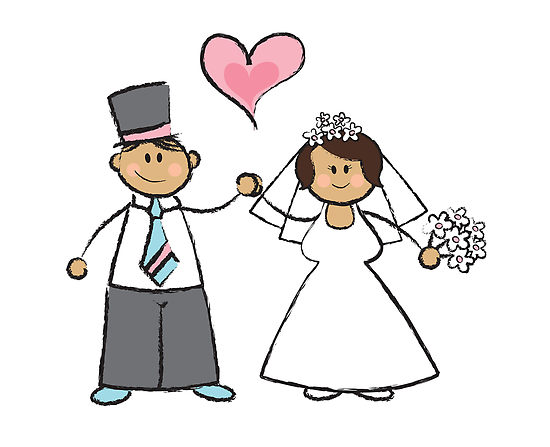
\includegraphics[scale=0.25]{gambar/just-married.jpg}
\end{center}
\newpage
\chap{Kompendium Katekese Gereja Katolik}
\setcounter{kgkcounter}{25}
{\normalsize

\kgk{Siapa saksi-saksi utama ketaatan iman dalam Kitab Suci?}
     Ada banyak saksi-saksi macam itu, secara khusus kita melihat dua. Yang 
pertama, Abraham, ketika mengalami ujian, dia tetap ``percaya kepada Allah''
(Rom 4:3) dan selalu taat kepada panggilan-Nya. Karena itulah Abraham disebut
          ``Bapa kaum beriman'' (Rom 4:11.18). Contoh yang kedua, Santa Perawan Maria
          yang seluruh hidupnya menjadi kesaksian sempurna ketaatan iman: ``Terjadilah
          padaku menurut perkataanmu'' (Luk 1:38).

\kgk{Apa artinya percaya kepada Allah bagi  seseorang dalam praktek
              hidupnya?}
Artinya, setia kepada Allah, mempercayakan hidup kepada-Nya, dan mengamini semua kebenaran yang diwahyukan Allah karena Allah adalah Kebenaran.
          Ini berarti percaya kepada satu Allah dalam tiga Pribadi, yaitu Bapa, Putra, dan Roh
          Kudus.

\kgk{Apa ciri-ciri iman?}
Iman adalah keutamaan adikodrati yang mutlak perlu bagi keselamatan. Iman
adalah anugerah cuma-cuma dari Allah dan tersedia bagi semua orang yang dengan
          rendah hati mencarinya. Tindakan iman adalah tindakan manusiawi, yaitu tindakan
          dari intelek manusia -- terdorong oleh kehendak yang digerakkan oleh Allah -- yang
          dengan bebas mengamini kebenaran ilahi. Iman juga pasti karena mempunyai dasar
          pada Sabda Allah, iman bekerja ``oleh kasih'' (Gal 5:6); dan iman berkembang terus-menerus dengan mendengarkan Sabda Allah dan doa. Dengan iman, bahkan
          sekarang ini juga, orang mencecap kegembiraan surga.

\kgk{Mengapa tidak ada kontradiksi antara iman dan ilmu?}
Walaupun iman itu mengatasi akal budi, tidak pernah ada kontradiksi antara
          iman dan ilmu karena kedua-duanya berasal dari Allah. Allah sendirilah yang
          memberikan, baik terang akal budi maupun terang iman kepada kita.

\flushright{(\dots \emph{bersambung} \dots)}
}
\end{document}